\documentclass[12pt, a4paper, ngerman]{article}
\title{AD-DA Wandler}
\author{Paul Walker \& Jens Hocke}
\date{29.09.2021}
\newcommand{\Autor}{Paul Walker \& Jens Hocke}
\newcommand{\Kurs}{INF20IN}
\newcommand{\MatrikelNummer}{}
\newcommand{\Was}{Laborbericht}
\newcommand{\Studiengang}{Informatik / Informationstechnik}

% \usepackage{biblatex} % für bibliografie
\usepackage{hyperref} % für links zum klicken
% \usepackage{color}    % für Farben (benötigt für listings)
% \usepackage{listings} % code schnipsel
\usepackage[ngerman]{babel} % lokalisierung der Titel (Inhaltsverzeichniss)
\usepackage{bookmark} % bookmarks für das PDF
\usepackage{csquotes} % korrekte quotes
\usepackage[version=3]{acro} % akronyme
\usepackage{geometry} % seitengeometrie (margin etc einstellen)
\usepackage{parskip}  % zeilenabstand bei neuem paragraph statt indentierung
\usepackage{fancyhdr} % header und footer
\usepackage{fontawesome5} % icons
% \usepackage{array}    % für bessere Tabellen
\usepackage{titlesec} % um die Titel anzupassen
\usepackage{graphicx} % für graphiken
\usepackage{pgfplots} % für plots

\graphicspath{{./assets/}}
\pgfplotsset{ table/search path={./assets/}}

\hypersetup{
  pdfauthor={\Autor},
  pdftitle={\Was},
  hidelinks
}

\geometry{
  a4paper,
  left=25mm,
  right=25mm,
  headheight=125mm,
  top=35mm,
  bottom=30mm,
  footskip=15mm
}

% title setup 
% make paragraph have a newline
\titleformat{\paragraph}
{\normalfont\normalsize\bfseries}{\theparagraph}{1em}{}
\titlespacing*{\paragraph}
{0pt}{3.25ex plus 1ex minus .2ex}{1.5ex plus .2ex}

% add bibliography (should we need one)
% \addbibresource{bibliography.bib}

% header and footer setup
\pagestyle{fancy}
\fancyhf{}
\rhead{\Was}
\lhead{\leftmark}
\lfoot{Autoren: \Autor, Kurs: \Kurs}
\rfoot{Seite \thepage}
\renewcommand{\headrulewidth}{1pt}
\renewcommand{\footrulewidth}{1pt}
\fancypagestyle{simple}{
  \fancyhf{}
  \rhead{\Was}
  \lfoot{Autor: \Autor, Kurs: \Kurs}
  \rfoot{Seite \thepage}
}

% acronyms
\acsetup{
  list/display = used,
  pages/display = first
}
\DeclareAcronym{adc}{short=ADC, long=Analog Digital Converter}
\DeclareAcronym{dac}{short=DAC, long=Digital Analog Converter}
\DeclareAcronym{inl}{short=INL, long=Integrale Nichtlinearität}
\DeclareAcronym{dnl}{short=DNL, long=Differenzielle Nichtlinearität}
\DeclareAcronym{dmm}{short=DMM, long=Digitales Multimeter}
\DeclareAcronym{ttl}{short=TTL, long=Transistor Transistor Logik}
\DeclareAcronym{fsr}{short=FSR, long=Full Scale Range}
\DeclareAcronym{op}{short=OpAmp, long=Operationsverstärker}
\DeclareAcronym{led}{short=LED, long=Light Emitting Diode ,first-style=short,subsequent-style=short}

\begin{document}

% Titlepage
\makeatletter
\begin{titlepage}
  \begin{center}
    \vspace*{1cm}
    {\Huge\scshape \Was}\\[2cm]
    \begin{center}
      \linespread{1}\Huge \@title\\[2cm]
    \end{center}
    {\large Studiengang \Studiengang}\\
    {\large an der Dualen Hochschule Baden-Württemberg\\ Stuttgart}\\[2cm]
    {\large von}\\
    {\large\bfseries \@author}
    \vfill
  \end{center}
\end{titlepage}
\makeatother

% Table of content
\tableofcontents

\newpage
\thispagestyle{simple}
\printacronyms[name=Abkürzungsverzeichnis, heading=section*]
\newpage

\section{Versuch Nr.1}

Es soll die \ac{inl} und die \ac{dnl} im mittleren Bereich,
sowie die Konversionsrate des \ac{adc} gemessen werden.

\subsection{Genutze Geräte und Bauteile}

\ac{dmm}: FLUKE 87 V True RMS Multimeter \\
Netzgerät: BASETech BT-153 \\
\ac{adc}: ADC0804 (National Semiconductor)

\subsection{Versuchsaufbau}

\begin{figure}%[h]
  \centering
  \begin{minipage}[b]{0.49\textwidth}
    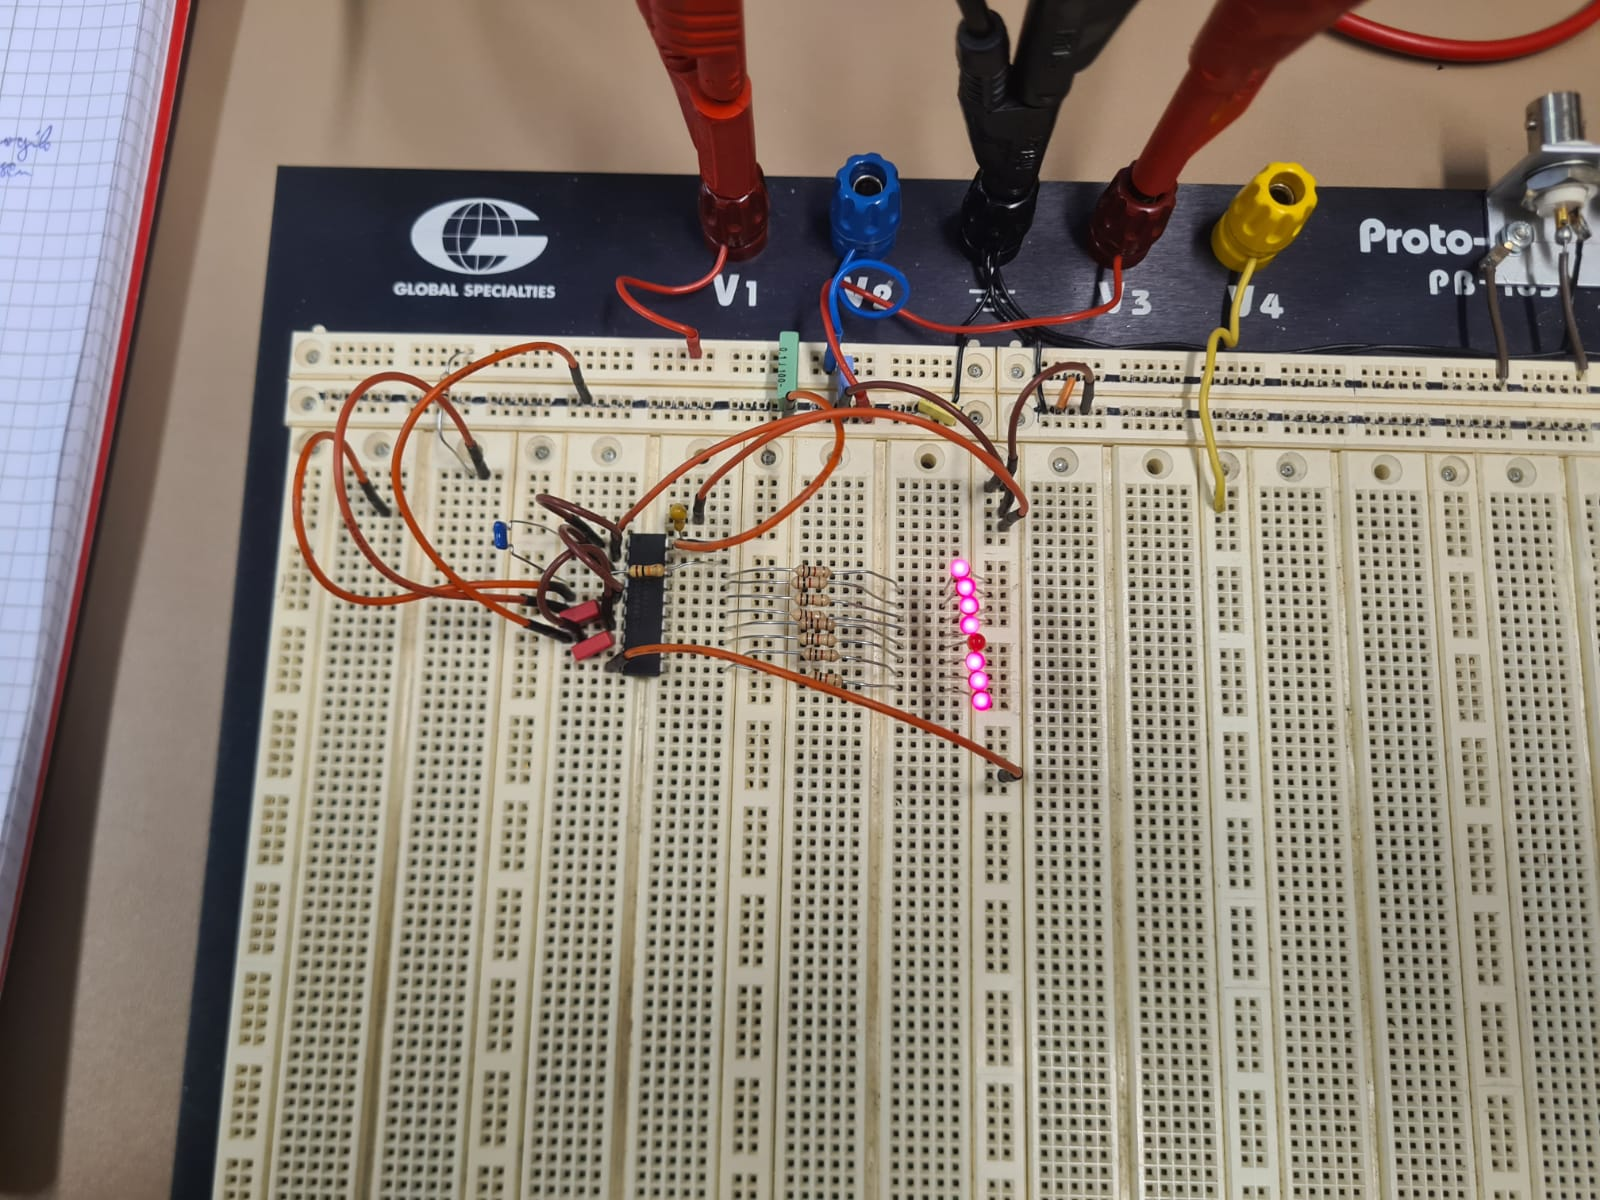
\includegraphics[width=\textwidth]{versuch_1_versuchsaufbau.jpeg}
    \caption{Versuchsaufbau}
    \label{abb:aufbau1}
  \end{minipage}
  \hfill
  \begin{minipage}[b]{0.49\textwidth}
    %TODO schaltskitze einfügen
    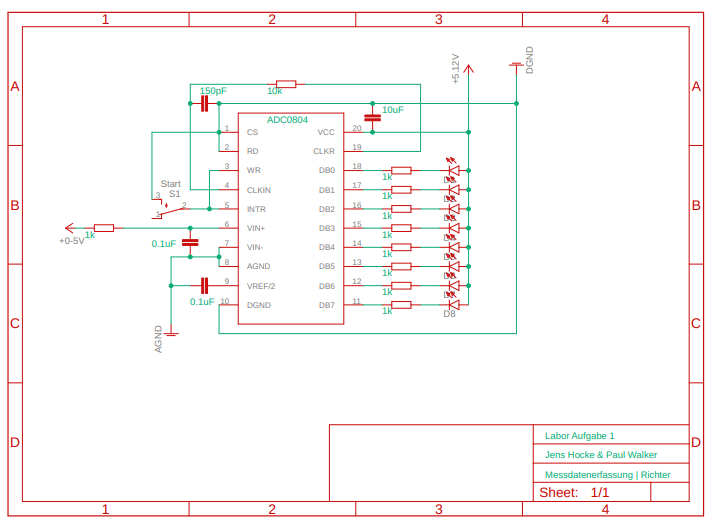
\includegraphics[width=\textwidth]{Schaltplan_Versuch_1.PNG}
    \caption{Schaltung}
    \label{abb:schaltung1}
  \end{minipage}
\end{figure}

Dafür wird die Schaltung in Abbildung \ref{abb:schaltung1}
und der Versuchsaufbau in Abbildung \ref{abb:aufbau1} verwendet. \\
Dabei ist zu beachten, dass der analoge Masseanschluss und der digitale Masseanschluss des \ac{adc}
bis zum Netzgerät getrennt verlaufen sollten, um Störungen zu vermeiden. \\
Für unsere Anwendung wird eine Referenz/Versorgungsspannung von $5.12V$ gewählt, um eine Auflösung von $20mV/LSB$ zu erreichen.
Um die Eingangsspannung möglichst genau einzustellen wird sie direkt am Netzgerät mit dem \ac{dmm} überprüft.
Auf dem Referenzschaltplan des Datenblattes das \ac{adc} ist der $V_{ref}/2$ Eingang
des \ac{adc} zusätzlich beschaltet. Dieser erhöht die Genauigkeit der Schaltung. %TODO sicher dass dadurch die genauigkeit erhöt wird?
Für unsere Anwendung wird er allerdings nicht benötigt.

Der \ac{adc} hat einen differenziellen analog Eingang.
Da in unserer Schaltung aber nur eine einfache analoge Eingangsspannung digitalisiert werden soll,
wird der negative Differenzielle Eingang $V_{IN}(-)$ auf GND gesetzt und $V_{IN}(+)$ als einfacher analoger Eingang verwendet.
Die analoge Eingangsspannung wird für den Versuch direkt vom Netzgerät bezogen
und für bessere Genauigkeit am Netzgerät mit einem \ac{dmm} gemessen.

Die Logik Ausgänge des \ac{adc} sind low-aktive \ac{ttl} Ausgänge.
Dadurch wird ein 1 Bitwert von einer nicht leuchtenden und ein 0 Bitwert von einer leuchtenden \ac{led} symbolisiert.
Die \ac{led}s können auch nicht umgekehrt beschalten werden, da das zu Störungen im \ac{adc} führen würde.

\subsection{Messung}

\subsubsection{\acl{inl}}\label{sec:inl}

Es soll die \ac{inl} des \ac{adc} über den gesamten Bereich gemessen werden.
Es werden 16 gleich große und in der \ac{fsr} gleichmäßig verteilte Übergänge des Bitmusters gemessen.

Dafür wird die analoge Eingangsspannung mit dem \ac{dmm} gemessen und protokolliert.
Daraufhin wird sie erhöht bis der nächste Bit-Sprung geschieht.
Der wert bei dem der Bit-Sprung auftritt, wird auch gemessen und protokolliert.

\begin{table}%[h]
  \centering
  \begin{tabular}{|c|c|c|c|}
    \hline
    Digital              & $V_{in}$                   & $\Delta V_{in}$ & Abweichung von der Idealgeraden \\\hline
    $15\rightarrow 16$   & $0,31V\rightarrow 0,316V$  & $6mV$           & $10mV\;;\;-4mV$                 \\\hline
    $31\rightarrow 32$   & $0,612V\rightarrow 0,636V$ & $24mV$          & $-8mV\;;\; -4mV$                \\\hline
    $47\rightarrow 48$   & $0,935V\rightarrow 0,953V$ & $18mV$          & $-5mV\;;\; -7mV$                \\\hline
    $63\rightarrow 64$   & $1,25V\rightarrow 1,27 V$  & $20mV$          & $-10mV\;;\;-10mV$               \\\hline
    $79\rightarrow 80$   & $1,575V\rightarrow 1,595V$ & $20mV$          & $-5mV\;;\; -5mV$                \\\hline
    $95\rightarrow 96$   & $1,887V\rightarrow 1,91 V$ & $23mV$          & $-13mV\;;\;-10mV$               \\\hline
    $111\rightarrow 112$ & $2,2V\rightarrow 2,215V$   & $15mV$          & $-20mV\;;\;-25mV$               \\\hline
    $127\rightarrow 128$ & $2,52V\rightarrow 2,54 V$  & $20mV$          & $-20mV\;;\;-20mV$               \\\hline
    $143\rightarrow 144$ & $2,837V\rightarrow 2,86 V$ & $23mV$          & $-23mV\;;\;-20mV$               \\\hline
    $159\rightarrow 160$ & $3,16V\rightarrow 3,18 V$  & $20mV$          & $-20mV\;;\;-20mV$               \\\hline
    $175\rightarrow 176$ & $3,476V\rightarrow 3,491V$ & $15mV$          & $-24mV\;;\;-29mV$               \\\hline
    $191\rightarrow 192$ & $3,79V\rightarrow 3,828V$  & $38mV$          & $-30mV\;;\;-12mV$               \\\hline
    $207\rightarrow 208$ & $4,115V\rightarrow 4,137V$ & $22mV$          & $-25mV\;;\;-23mV$               \\\hline
    $223\rightarrow 224$ & $4,428V\rightarrow 4,444V$ & $16mV$          & $-32mV\;;\;-36mV$               \\\hline
    $239\rightarrow 240$ & $4,74V\rightarrow 4,756V$  & $16mV$          & $-40mV\;;\;-44mV$               \\\hline
    $254\rightarrow 255$ & $5,046V\rightarrow 5,055V$ & $9mV$           & $-34mV\;;\;-45mV$               \\\hline
  \end{tabular}
  \caption{Werte}
  \label{table:1}
\end{table}

\begin{figure}%[h]
  \begin{tikzpicture}
    \begin{axis}[
        width=\textwidth,
        height=10cm,
        xmin=0,
        xmax=265,
        minor y tick num = 3,
        ymin=0,
        ymax=5.12,
        ylabel={Spannung in $V$},
        xlabel={Digitaler Ausgangswert}
      ]
      \addplot table[
          color=blue,
          col sep=semicolon,
          /pgf/number format/read comma as period,
          x=Dig,
          y=V
        ]{data_versuch_1_2.csv};
      \addlegendentry{Messwerte}
      \addplot [
        domain=0:255,
        samples=10,
        color=red,
      ]
      {x*0.02};
      \addlegendentry{Idealgerade}
    \end{axis}
  \end{tikzpicture}
  \caption{Übertragungskennlinie \ac{inl}}
  \label{plot:inl}
\end{figure}

\begin{figure}%[h]
  \begin{tikzpicture}
    \begin{axis}[
        ybar interval,
        ymax=40,
        ymin=0,
        xmin=16,
        xmax=256,
        minor y tick num = 3,
        width=\textwidth,
        height=10cm,
        xlabel={Digitaler Output},
        ylabel={Differenzspannungen in $mV$}
      ]
      \addplot table [x=Dig2, y=dmV, col sep=semicolon, /pgf/number format/read comma as period] {data_versuch_1.csv};
    \end{axis}
  \end{tikzpicture}
  \caption{Differenzspannungen \ac{inl}}
  \label{plot:diff1}
\end{figure}


In Abbildung \ref{plot:inl} und in Tabelle \ref{table:1} lässt sich ein gain Fehler feststellen.
Dieser Fehler kann vom Bauteil kommen oder aber von einer falschen Einstellung von $V_{ref}$.
Korrigieren lässt sich der Fehler durch Anpassen von $V_{ref}$. \\
Massive Fehler in den Differenzspannungen sind nicht erkennbar,
der Wert liegt wie erwartet überall bei etwa $20mV$ (siehe Abbildung \ref{plot:diff1})

\subsubsection{\acl{dnl}}

Es soll die \ac{dnl} über den mittleren Bereich des \ac{adc} gemessen werden.
Dazu werden neun symmetrisch um die Bereichsmitte liegende Werte gemessen.
Das Messverfahren ist das gleiche wie in \ref{sec:inl}

\begin{figure}%[h]
  \begin{tikzpicture}
    \begin{axis}[
        width=\textwidth,
        height=10cm,
        xmin=123,
        xmax=133,
        ymin=2.4,
        ymax=2.7,
        xlabel={Digitaler Ausgangswert},
        ylabel={Spannung in $V$}
      ]
      \addplot table[
          color=blue,
          col sep=semicolon,
          /pgf/number format/read comma as period,
          y=V,
          x=Dig
        ]{data_versuch_1b.csv};
      \addlegendentry{Messwerte}
      \addplot [
        domain=124:132,
        samples=10,
        color=red,
      ]
      {x*0.02};
      \addlegendentry{Idealgerade}
    \end{axis}
  \end{tikzpicture}
  \caption{Übertragungskennlinie \ac{dnl}}
  \label{plot:dnl}
\end{figure}

\begin{figure}%[h]
  \begin{tikzpicture}
    \begin{axis}[
        ybar interval,
        ymax=40,
        ymin=0,
        xmin=124,
        xmax=132,
        minor y tick num = 3,
        width=\textwidth,
        height=10cm,
        xlabel={Digitaler Output},
        ylabel={Differenzspannungen in $mV$}
      ]
      \addplot table [x=Dig, y=Vdiff, col sep=semicolon, /pgf/number format/read comma as period] {data_versuch_1b_2.csv};
    \end{axis}
  \end{tikzpicture}
  \caption{Differenzspannungen \ac{dnl}}
  \label{plot:diff2}
\end{figure}

Es ist wie in \ref{sec:inl} ein Offsetfehler erkennbar (Abbildung \ref{plot:dnl}).
In den Differenzspannungen (Abbildung \ref{plot:diff2}) ist kein nennenswerter Fehler feststellbar.
Monotonieverletzungen sind auch nicht erkennbar (Abbildung \ref{plot:dnl}).

\subsubsection{Konversionszeit}

Die Clock-Frequenz des \ac{adc} kann über die Clock-Pins des \ac{adc} gemessen werden und beträgt $418kHz$

Die Konversionszeit kann direkt am Interrupt Eingang gemessen werden,
da der \ac{adc} in unserem Fall im \enquote{Free Running Mode} arbeitet
und damit maximal schnell konvertiert.
Die Konversionsrate beträgt $5,87kHz$ und die Konversionszeit damit $170,3\mu s$

Damit benötigt der \ac{adc} $71$ Clock-Zyklen zum Konvertieren eines Wertes.

%TODO vergleich mit Datenblatt

\section{Versuch Nr.2}

Es soll die Monotonie, die Linearität und die Einschwingzeit des \ac{dac} gemessen werden.

\subsection{Genutzte Geräte und Bauteile}

\acl{dmm}: FLUKE 87 V True RMS Multimeter \\
Netzgerät: BASETech BT-153 \\
Funktionsgenerator: Tektronix AFG3022 Dual Channel Arbitrary/Function Generator \\
Oszilloskop: Keysight DSOX1102A Digital Storage Oscilloscope \\
\ac{dac}: DAC ZN429 (Ferranti)
% TODO hier vielleicht noch den DFlipFlop hinzufügen

\subsection{Versuchsaufbau}


\begin{figure}%[h]
  \centering
  \begin{minipage}[b]{0.49\textwidth}
    \includegraphics[width=\textwidth]{versuch_2_versuchsaufbau.jpg}
    \caption{Versuchsaufbau}
    \label{abb:aufbau2}
  \end{minipage}
  \hfill
  \begin{minipage}[b]{0.49\textwidth}
    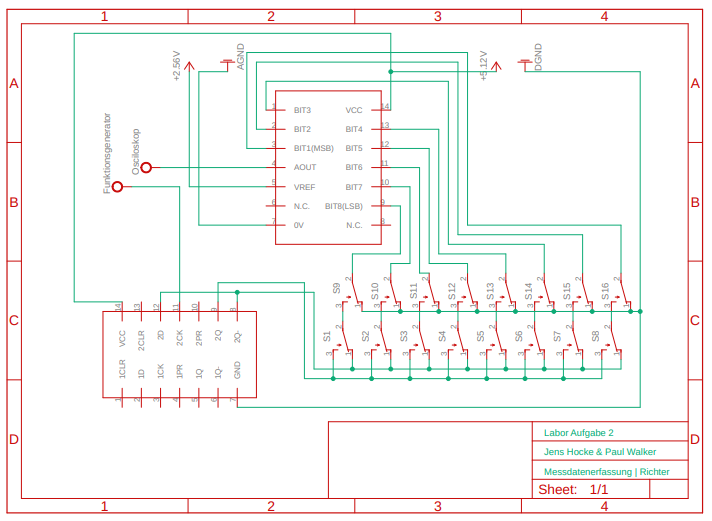
\includegraphics[width=\textwidth]{schaltplan_versuch_2.png}
    \caption{Schaltung}
    \label{abb:schaltung2}
  \end{minipage}
\end{figure}

Für die Messung wird die Schaltung in Abbildung \ref{abb:schaltung2}
und der Versuchsaufbau in Abbildung \ref{abb:aufbau2} verwendet. \\
Es ist zu beachten, dass der \ac{dac} eine Referenzspannung von $2,56V$
aber eine Versorgungsspannung von $5V$ benötigt.

Es wird der analoge Output des \ac{dac} mit dem Oszilloskop gemessen.
Die Messung wäre zwar auch mit einem \ac{dmm} möglich,
allerdings besitzt das Oszilloskop in dieser Anwendung eine höhere Genauigkeit, da eine Spannungsdifferenz gemessen werden soll.
Bei der Messung ist der Innenwiederstand nicht zu beachten, da dieser hochohmig ist.

\subsection{Messung}

Um die Monotonie und Nichtlinearität des \ac{dac} zu messen,
werden schrittweise Bitmusters, bei denen genau ein Bit gesetzt ist zwischen diesem und dem darunterliegenden muster gewechselt.
Dieser Sprung wird dann am Oszilloskop gemessen.

So werden alle Bit-Stellen Schritt für Schritt getestet.
% TODO: Statt der in der Literatur angegebenen Triggerung des Scope mit dem Q-Ausgagng des FF
% könnte auch direkt mit dem Bitsprung des DAC-Ausgangs getriggert werden. 
% Was ist vorzuziehen? Begründung? 

\begin{table}%[h]
  \centering
  \begin{tabular}{|c|c|c|c|}
    \hline
    Digital                            & $\Delta U_{out}$ & monoton?       \\\hline
    $0000\,0001\rightarrow 0000\,0000$ & $9,5mV$          & \faIcon{check} \\\hline
    $0000\,0010\rightarrow 0000\,0001$ & $9,5mV$          & \faIcon{check} \\\hline
    $0000\,0100\rightarrow 0000\,0011$ & $9,8mV$          & \faIcon{check} \\\hline
    $0000\,1000\rightarrow 0000\,0111$ & $9,675mV$        & \faIcon{check} \\\hline
    $0001\,0000\rightarrow 0000\,1111$ & $9,425mV$        & \faIcon{check} \\\hline
    $0010\,0000\rightarrow 0001\,1111$ & $9,5mV$          & \faIcon{check} \\\hline
    $0100\,0000\rightarrow 0011\,1111$ & $10,075mV$       & \faIcon{check} \\\hline
    $1000\,0000\rightarrow 0111\,1111$ & $12,25mV$        & \faIcon{check} \\\hline
    $0000\,0000\rightarrow 1111\,1111$ & $2,375V$         & \faIcon{check} \\\hline
  \end{tabular}
  \caption{Werte}
  \label{table:2}
\end{table}

Das Ergebnis ist eine gute Linearität mit $\Delta U_{out}\approx 10mV$.
Für eine Ideale Linearität werden für eine Auflösung von 8Bit bei einer Versorgungsspannung von $2.56V$
wird der Wert $10mV/LSB$ erwartet. Es wird noch von Linearität gesprochen so lange $\Delta U_{out}<2LSB$.
Damit ist der \ac{dac} sehr stark linear. \\
Die Messungen haben außerdem ergeben, dass der \ac{dac} durchgängig linear ist.
Denn ein positiver Bit-Sprung erzeugt in jedem Fall eine Positive $U_{out}$ Flanke.

\begin{figure}%[h]
  \centering
  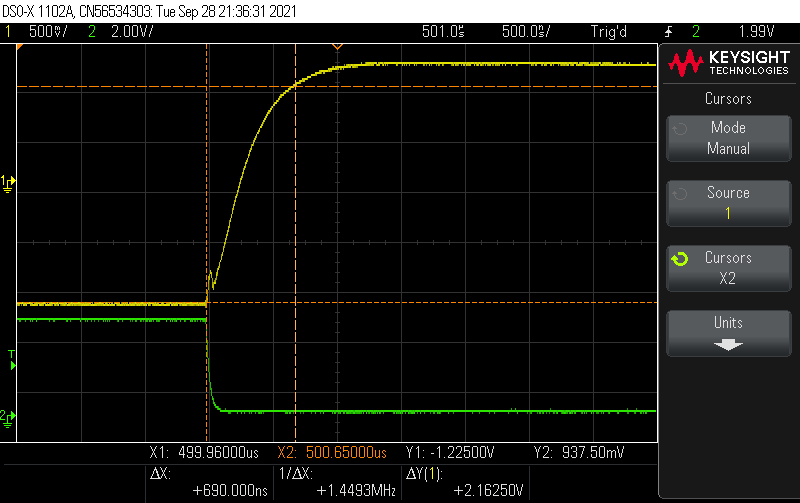
\includegraphics[width=0.6\textwidth]{scope_34.png}
  \caption{Einschwingverhalten}
  \label{abb:einschwing1}
\end{figure}

In Abbildung \ref{abb:einschwing1} ist das Einschwingverhalten des \ac{dac} für den Übergang $0000\,0000\rightarrow 1111\,1111$
dargestellt. Da sich bei diesem Bitmuster die alle Bits ändern und $\Delta U_{out}$ am höchsten ist,
ist es ideal für die Feststellung der Einschwingzeit. Die Zeit bis $10\%$ von $U_{out MAX}$ erreicht sind,
beträgt $90ns$. Die Zeit bis $90\%$ von $U_{out MAX}$ erreicht sind,
beträgt $690ns$ % TODO vergleich mit Datenblatt

% \printbibliography

\section{Versuch Nr.3}

Es soll der analoge Fehler der Hintereinanderschaltung von \ac{adc} und \ac{dac} gemessen werden.

\subsection{Genutzte Geräte und Bauteile}

\acl{dmm}: FLUKE 87 V True RMS Multimeter \\
Netzgerät 1: BASETech BT-153 \\
Netzgerät 2: PeakTech DC Dual Power Supply 6210 \\
Funktionsgenerator: Tektronix AFG3022 Dual Channel Arbitrary/Function Generator \\
Oszilloskop: Keysight DSOX1102A Digital Storage Oscilloscope \\
\ac{dac}: DAC ZN429 (Ferranti) \\
\ac{adc}: ADC0804 (National Semiconductor)
% TODO hier vielleicht noch den OpAmp hinzufügen

\subsection{Versuchsaufbau}

\begin{figure}%[h]
  \centering
  \begin{minipage}[b]{0.49\textwidth} % TODO Versuchsaufbau hinzufügen
    \includegraphics[width=\textwidth]{example-image-a}
    \caption{Versuchsaufbau}
    \label{abb:aufbau3}
  \end{minipage}
  \hfill
  \begin{minipage}[b]{0.49\textwidth}
    \includegraphics[width=\textwidth]{example-image-b}
    \caption{Schaltung}
    \label{abb:schaltung3}
  \end{minipage}
\end{figure}

Für die Messung wird die Schaltung in Abbildung \ref{abb:schaltung3}
und der Versuchsaufbau in Abbildung \ref{abb:aufbau3} verwendet. \\
Diese Schaltung liefert als Ausgangsspannung den Fehler
der Hintereinanderschaltung von \ac{adc} und \ac{dac}.
Dabei sollen allerdings nur Differenzfehler gemessen werden,
Offsetfehler sollen nicht betrachtet werden.
Daher muss die Verstärkerschaltung nach dem \ac{dac} einstellbar gemacht werden.
Dies geschieht über ein Potenziometer.
Als Ausgangswert wird die Verstärkerschaltung über das Potenziometer auf eine Verstärkung von $4$ gesetzt.
Damit werden auch die unterschiedlichen Arbeitsspannungen des \ac{adc} und \ac{dac} und der Innenwiederstand des \ac{dac} ausgeglichen.

Es werden insgesamt 3 Versorgungsspannung benötigt.
Der \ac{dac} benötigt $5V$ Versorgungsspannung und $2,56V$ Referenzspannung.
Der \ac{adc} benötigt $5,12V$ Versorgungs-/Referenzspannung.
Der \ac{op} benötigt $\pm 14V$ Versorgungsspannung.


\subsection{Messung}

\subsubsection{Analog Error Signal}

Es wird der Fehler der Hintereinanderschaltung des \ac{adc} und \ac{dac} am Ausgang gemessen.

\begin{figure}
  \centering
  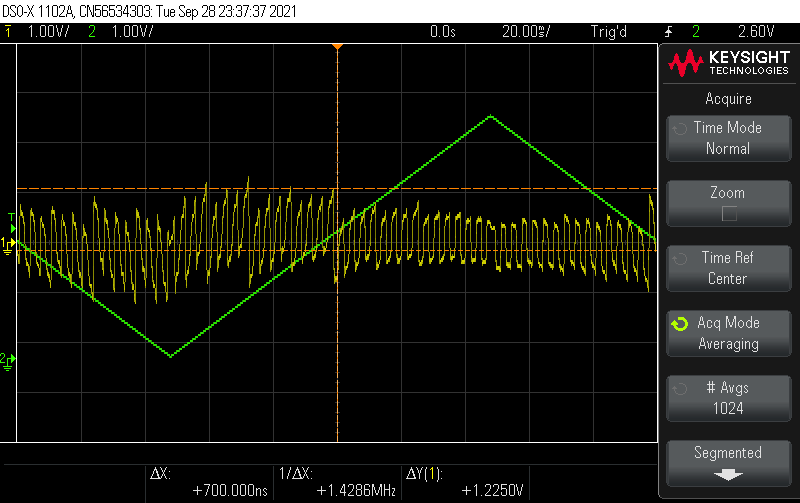
\includegraphics[width=0.7\textwidth]{scope_38.png}
  \caption{Fehler der Schaltung}
  \label{plot:fehler1}
\end{figure}

In Abbildung \ref{plot:fehler1} ist erkennbar,
dass das Fehlersignal in etwa horizontal und gleichmäßig verläuft.

Aus diesem Fehlersignal kann der Fehler des \ac{adc} ungefähr bestimmt werden,
da dieser den größten Einfluss auf den Fehler hat. \\
Der Fehler des \ac{adc} kann mit dieser Formel aus dem Output der Schaltung bestimmt werden.
Aufgrund der 10-Fachen Verstärkung muss $\Delta U$ durch $10$ geteilt werden.

$$
  Fehler ADC \approx (\frac{\frac{\Delta U}{10}}{20mV})_{LSB}-1 = (\frac{\frac{1,45V}{10}}{20mV})_{LSB} = \pm 6 LSB
$$

\subsubsection{Aliasing Effekt}

Nun wird das Signal direkt am Ausgang des \ac{dac} gemessen und mit dem Eingangssignal verglichen.
Dabei fällt auf, dass es bei hohen Frequenzen am Ausgang immer schwerer wird verschiedene Signale zu unterscheiden.

\begin{figure}%[h]
  \centering
  \begin{minipage}[b]{0.49\textwidth} % TODO Versuchsaufbau hinzufügen
    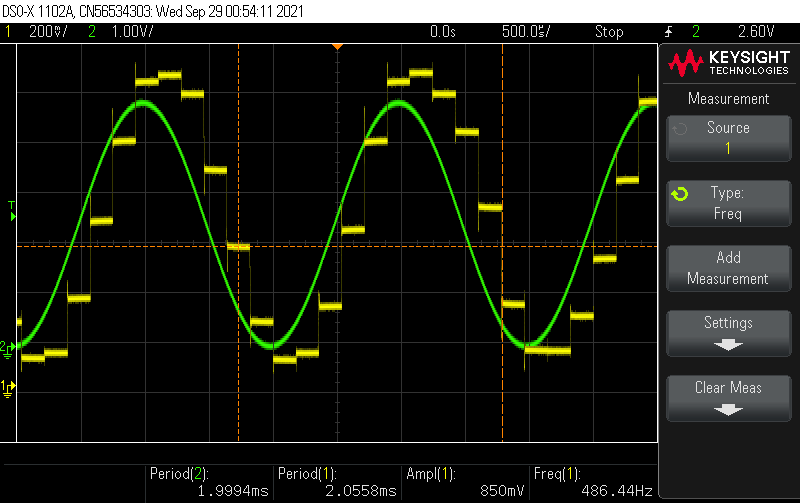
\includegraphics[width=\textwidth]{scope_49.png}
    \caption{Sinus Signal}
    \label{abb:aliasSin}
  \end{minipage}
  \hfill
  \begin{minipage}[b]{0.49\textwidth}
    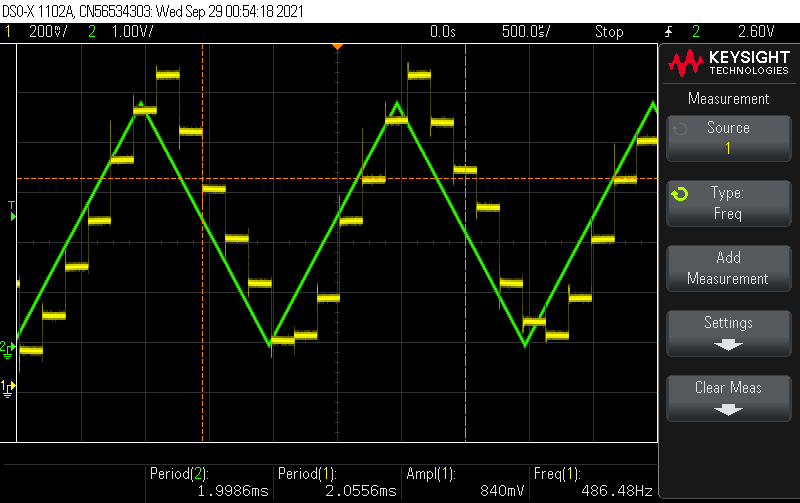
\includegraphics[width=\textwidth]{scope_50.png}
    \caption{Dreieck Signal}
    \label{abb:aliasTri}
  \end{minipage}
\end{figure}

So Lässt sich ab etwa $500Hz$ fast kein Unterschied
zwischen einem Sinus Signal (Abbildung \ref{abb:aliasSin})
und einem Dreieck Signal (Abbildung \ref{abb:aliasTri}) finden.

Grundsätzlich kann man sagen,
dass Signale ab der halben Abtastfrequenz aufwärts nicht mehr unterscheidbar sind.
Es entstehen Schwebungszustände. Man spricht auch vom Nyquist-Kriterium.


\end{document}